\section{Introducción}
\setcounter{sectiontotal}{3}

\begin{frame}
\frametitle{\pagetitle}
\framesubtitle{Descripción}
\begin{figure}
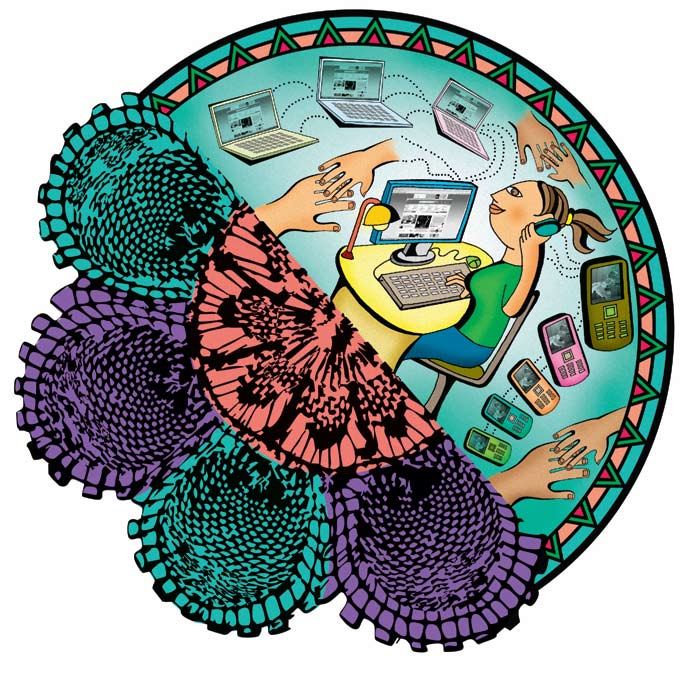
\includegraphics[scale=.3]{imagenes/nhanduti}
\end{figure}
\end{frame}

\begin{frame}
\frametitle{\pagetitle}
\framesubtitle{Objetivo general}
\begin{block}{Descripción}
\centering
Identificar y valorar los aspectos pedagógicos, de diseño, de implementación y
de evaluación que influyen a la creación de herramientas educativas que utilizan
las corrientes pedagógicas actuales apoyadas en las TIC, especialmente los
juegos serios.
\end{block}


\end{frame}

\begin{frame}
\frametitle{\pagetitle}
\framesubtitle{Objetivos específicos}

\small
\begin{itemize}[<+->]
\item Proveer una visión actualizada de las corrientes pedagógicas apoyadas con las TIC.
\item Proveer una visión actualizada de los juegos serios.
\item Identificar áreas de aplicación de los juegos serios.
\item Seleccionar las herramientas tecnológicas disponibles para el desarrollo de juegos serios.
\item Contrastar en la práctica los conocimientos teóricos adquiridos a través del diseño
e implementación de un juego serio.
\item Evaluar la solución propuesta para identificar los
aspectos de diseño, desarrollo y evaluación de los juegos serios.
\end{itemize}
\end{frame}

